
\chapter{Modeling} \label{ch:modeling}

In order to model the contact between the \gls{ee}'s tactile sensors, eight different model categories are present\cite*{articulated-hands-force-control-and-kinematic-issues} whereas three most common ones within the field of robotics\cite[Chapter 37]{handbook-of-robotics} are \gls{pwof}, \gls{hf} and the \gls{sf} model as shown in \figref{fig:contact-models}. \medskip

\begin{figure}[h]
	\centering
	\begin{subfigure}[b]{0.3\textwidth}
		\centering
		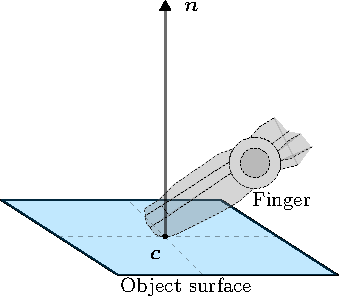
\includegraphics[width=\textwidth]{chapters/modeling/fig/contact-no-friction.pdf}
		\caption{Point contact model without friction.}
		\label{fig:pwof}
	\end{subfigure}
	\hfill
	\begin{subfigure}[b]{0.3\textwidth}
		\centering
		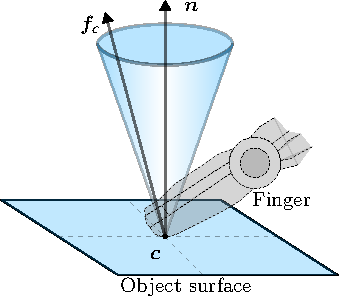
\includegraphics[width=\textwidth]{chapters/modeling/fig/hf.pdf}
		\caption{Point contact model with friction.}
		\label{fig:hf}
	\end{subfigure}
	\hfill
	\begin{subfigure}[b]{0.3\textwidth}
		\centering
		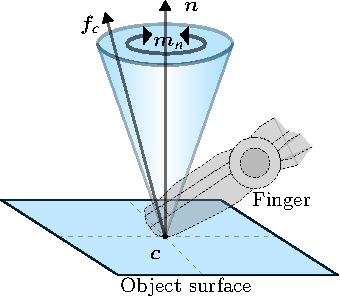
\includegraphics[width=\textwidth]{chapters/modeling/fig/sf.pdf}
		\caption{Soft-finger model.}
		\label{fig:sf}
	\end{subfigure}
	   \caption{The three most commonly used contact models.}
	   \label{fig:contact-models}
\end{figure}

% no friction
The \gls{pwof} model, as shown in \figref{fig:pwof}, can only represent forces along with the normal of the object's surface at the point of contact and thus the model does not support surface deformations between the two contacting objects. This model is applied in cases where very little deformation is present, along with the contact being slippery\cite[Chapter 38]{handbook-of-robotics}.\medskip

% Hard finger
The \gls{hf} model, as shown in \figref{fig:hf}, is representative when the friction between objects is great enough to be significant, while the contact deformation is small enough to ignore friction moments and deformations\cite[Chapter 38]{handbook-of-robotics}. To model the friction acting on the contact point a great number of methods exist, a very common one being the Column friction with different modifications depending on the use case\cite*{modelling-of-joint-friction-in-robotic-manipulators-with-gear-transmissions}. \medskip

% Soft finger
The \gls{sf} model, as shown in \figref{fig:sf}, is used to represent scenarios where both friction and surface deformations are great enough to be impactful in the systems behavior. Due to deformations of the finger an additional torsional moment about the contact normal will be present\cite[Chapter 38]{handbook-of-robotics}. \medskip

Based on the contact model categories described above, the most representative is \gls{sf} since these models can provide descriptions of the contact surface topology, and thus enable the solving of the \gls{iep} by deriving surface features for pose estimation. Furthermore in order to manipulate objects in-hand and ensuring force closure modeling friction is crucial, which is also provided by these models. An illustration of the system as a \gls{sf} with friction cone and pressure distribution can be seen in \figref{fig:friction-contact-distribution}, while \figref{fig:force-closure-model} shows the model enabling force closure about the object $\{O\}$, where the external force is represented as gravity which is a common occurrence.

\begin{center}
    \renewcommand{\arraystretch}{1.2}
    \begin{minipage}{.48\linewidth}
        \vspace{0pt}
        \centering
        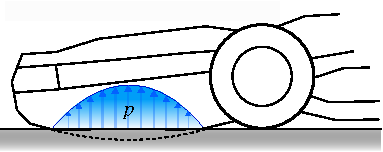
\includegraphics[width=.95\textwidth]{chapters/modeling/fig/contact-surface.pdf}%
        \vspace{0.6cm}
        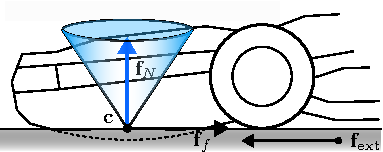
\includegraphics[width=.95\textwidth]{chapters/modeling/fig/friction-cone-schematic.pdf}%
    \end{minipage}%
    \hfill%
    \begin{minipage}{.48\linewidth}
        \vspace{0pt}
        \centering
        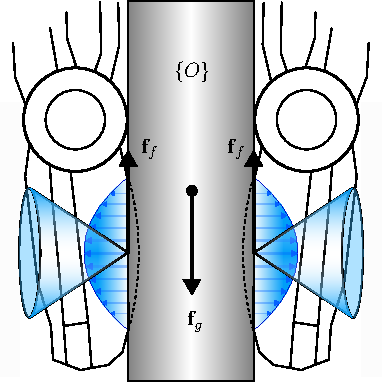
\includegraphics[width=.95\textwidth]{chapters/modeling/fig/force-closure-contact.pdf}
    \end{minipage}%
    %    
    \vspace{15pt}
    %
    \begin{minipage}[t]{.48\linewidth}
        \vspace{0pt}
        \captionsetup{type=figure}
        \captionof{figure}{Contact pressure distribution and friction cone for a \gls{sf} model in the context of a robotic finger.}
        \label{fig:friction-contact-distribution}
    \end{minipage}%
    \hfill%
    \begin{minipage}[t]{.48\linewidth}
        \vspace{0pt}
        \captionsetup{type=figure}
        \captionof{figure}{Contact pressure distribution and friction cone causing force closure to prevent the object $\{O\}$ from falling due to gravity.}
        \label{fig:force-closure-model}
    \end{minipage}%
\end{center}

Within these figures $p(r)$ is the pressure distribution often as a function of the contact surface's radius $r$ assuming a non-conforming contact case. $\mathbf{f}_N$ is the normal force of the object acting on the \gls{ee} in the contact point $\mathbf{c}$, $\mathbf{f}_f$ is the friction force opposing the external force $\mathbf{f}_{\text{ext}}$ which often comes in the form of gravity $\mathbf{f}_g$ as see in \figref{fig:force-closure-model}.

% make the object identical to the one in the previous figure + finger tip contour from contact models

\begin{figure}[h]
	\begin{small}
		\begin{center}
			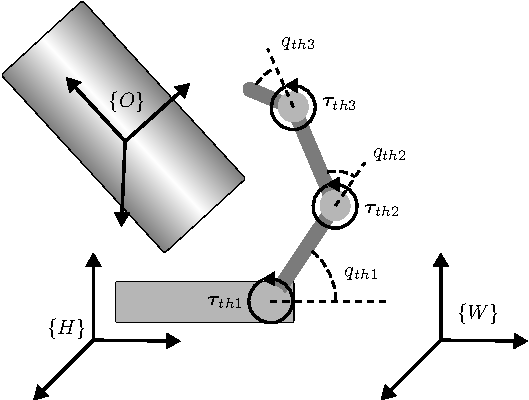
\includegraphics[width=0.8\textwidth]{chapters/modeling/fig/kinematic-tree-manipulator.pdf}
		\end{center}
		\caption{The model of the world representation for this project.}
		\label{fig:full-system-model}
	\end{small}
\end{figure}

With the contact model described, a segment of the kinematic tree of the \gls{ee} can be seen in \figref{fig:full-system-model}. Here $q_{thi}$ is the angle of the $i$'th joint in the thumb which here is the only finger depicted, $\boldsymbol{\tau}_{thi}$ is the torque exerted by said joint, $\{W\}$ is the world frame, $\{O\}$ is the object's frame and $\{H\}$ is the robotic hand's frame. While only a single finger here is illustrated the naming conventions and representations simply scale to all the \gls{ee}'s \gls{dof}s.


To determine which methods best describe the models presented above for this project, the \gls{sota} will be presented in \chapref{ch:state-of-the-art}.